\begin{appendix}


\section{Anhang}

\begin{figure}
  \centering
  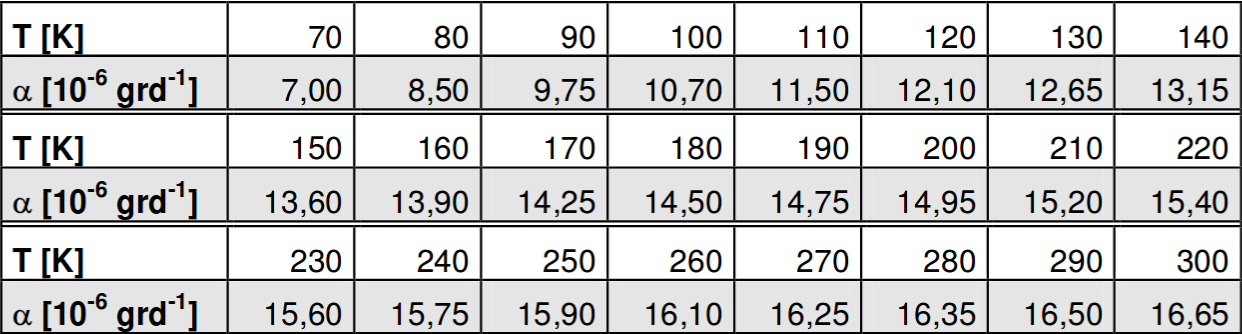
\includegraphics[width=\textwidth]{ressources/alpha.png}
  \caption{Ausdehnungskoeffizient $\alpha$ von Kupfer in Abhängigkeit von der Temperatur $T$. \cite{skript}}
  \label{fig:alphaa}
\end{figure}

\begin{figure}
  \centering
  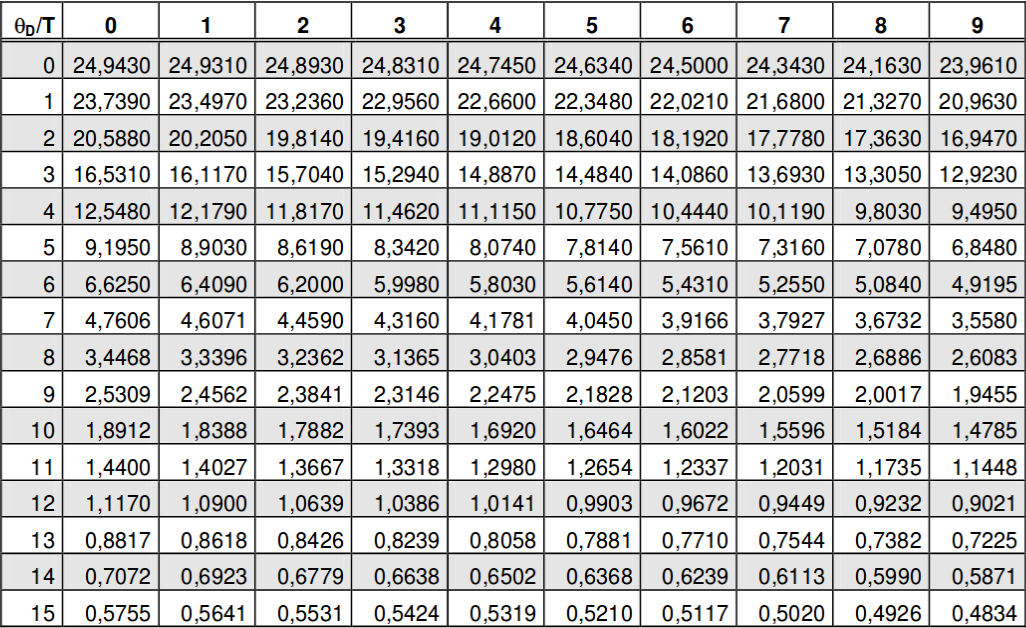
\includegraphics[width=\textwidth]{ressources/hugetable.png}
  \caption{Werte der Wärmekapazität aus der Debyefunktion in Abhängigkeit von der Debye-Temperatur $\Theta_\text{D}$ und der Temperatur $T$. \cite{skript}}
  \label{fig:mirfallenkeinelabelmehreinfuerdenganzenmistfuckthisshitimoutwarumtueichmirdasanundesistschonhalbzweinachtsdafuq}
\end{figure}
% \centering
% \begin{figure}
% \includepdf[width=0.9\textwidth, pages={1}]{Bilder/Messdaten.pdf}
% \end{figure}
% \newpage
% \begin{figure}
% \includepdf[width=0.9\textwidth, pages={2}]{Bilder/Messdaten.pdf}
% \end{figure}
%
\end{appendix}
